\mysubsection{Programmation distribuée}

\ifslide{
  \begin{frame}{Une longue et vielle histoire...}
   \begin{block}{Historique}
     \begin{itemize}
       \item DCE
       \item CORBA
       \item Java-RMI
       \item COM/DCOM
       \item EJB
       \item ...
     \end{itemize}
   \end{block}
  \end{frame}

  \begin{frame}{Enjeu}
   \begin{block}{Motivation}
     \begin{itemize}
       \item séparer le code entre différente instance physique
       \item tenu de charge, routage, balance de charge
       \item sécurité
     \end{itemize}
   \end{block}
  \end{frame}

  \begin{frame}{Remote Procedure Call}
    \begin{block}{Qu'est ce que RPC ?}
      \begin{itemize}
        \item base de nombreuses technologies (DCE, DCOM/COM,...)
        \item idée ancienne (1976)
        \item \mylink{http://tools.ietf.org/html/rfc707}{RFC 707}
      \end{itemize}
    \end{block}

    \begin{block}{Avantages/Inconvénients}
      \begin{itemize}
        \item Indépendance du transport
        \item Transformation des données
        \item Bloque le Client lors d’un appel à une procédure
        \item Echec possible en cas de problèmes réseaux
        \item Gestion difficile de reprise d’erreur
      \end{itemize}
    \end{block}
  \end{frame}

  \begin{frame}{MOM vs RPC}
    \begin{center}
      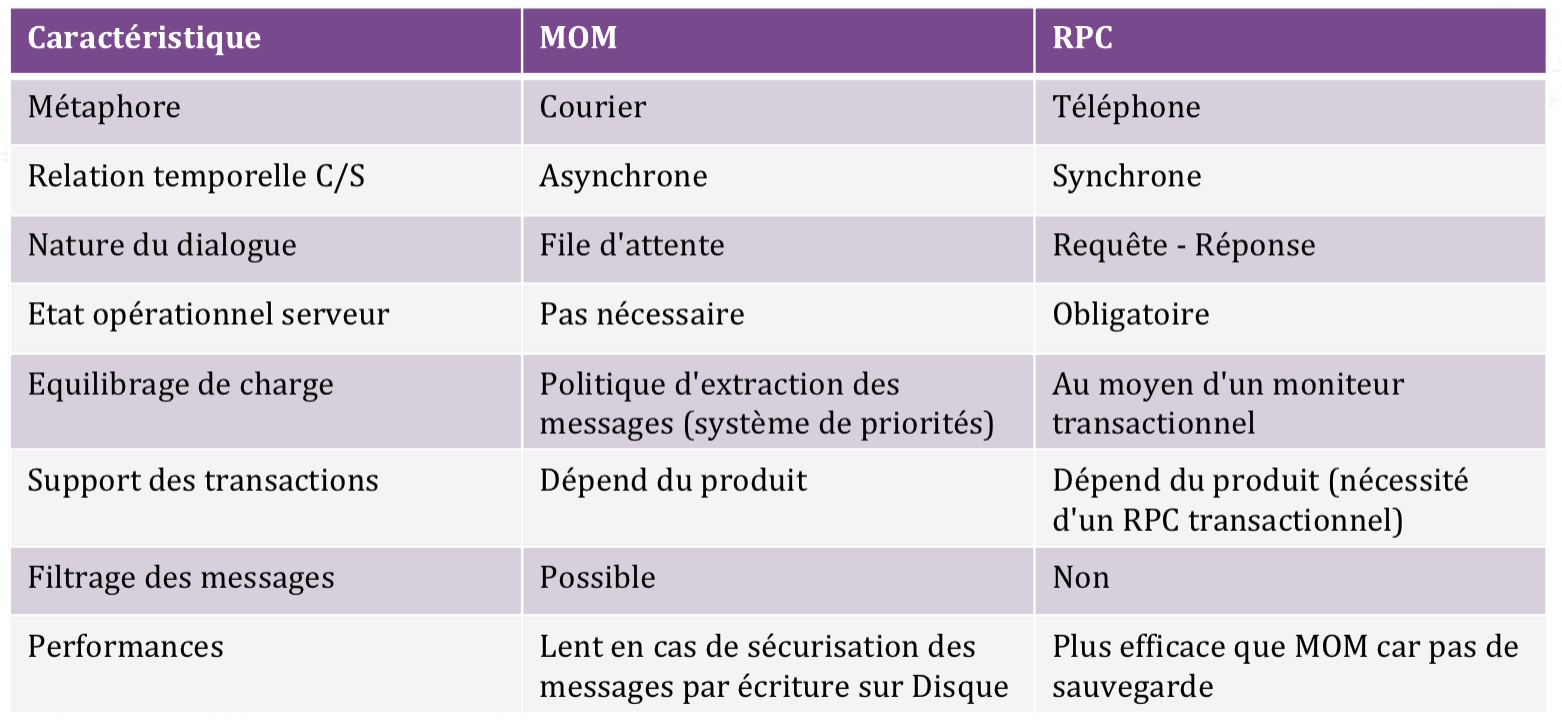
\includegraphics[scale=0.22]{img/mom-rpc.png}
    \end{center}
  \end{frame}

  \begin{frame}{Middleware orientés objets}
   \begin{block}{Motivation}
     \begin{itemize}
       \item invoqué des objets à distances (plutôt que récupérer des données)
       \item ex: DCE, DCOM, RMI, SOAP,...
     \end{itemize}
    \end{block}
  \end{frame}

  \begin{frame}{Ex: Java RMI}
    \begin{block}{Remote Method Invocation}
     \begin{itemize}
       \item originellement interopérable que entre machines virtuelles
       \item protocole sous jacent Java Remote Method Protocole (JRMP)
       \item étendu pour supporter CORBA (interopérabilité hors Java) : RMI-IIOP
     \end{itemize}
    \end{block}

    \begin{center}
      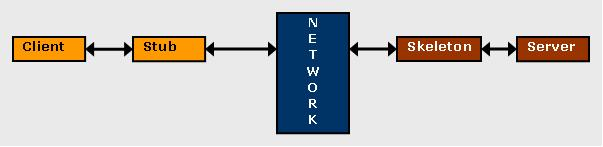
\includegraphics[scale=0.6]{img/rmi-stubs-skeletons.jpg}
    \end{center}
  \end{frame}

}
